\documentclass{article}

% Language setting
\usepackage[english]{babel}

% Set page size and margins
\usepackage[letterpaper,top=1.8cm,bottom=1.8cm,left=2.2cm,right=2.2cm,marginparwidth=1.5cm]{geometry}

% Useful packages
\usepackage{amsmath}
\usepackage{graphicx}
\usepackage[colorlinks=true, allcolors=blue]{hyperref}
\usepackage{booktabs}
\usepackage{algorithm}
\usepackage{algpseudocode}
\usepackage{multirow}
\usepackage{enumitem}
\usepackage{float}

\title{Inverse Physics Learning from Camera Projections:\\Observability, Dual-Parameter Recovery, and\\Noise Robustness in MPM Material Identification}

\author{Your Name}

\begin{document}
\maketitle

% ==============================================================================
\begin{abstract}
Inferring material parameters from observed deformation is a core challenge
in computational mechanics.  This paper presents a comprehensive study of
neural-network-based inverse physics learning under different observation
spaces, parameter counts, and noise conditions.  We evaluate three training
architectures---Baseline (3D observable, finite-difference), Camera (2D
projected observable, finite-difference), and Full Autodiff---across four
experimental sections: (1)~Clean 3D observables with $E^*=400$, where the
FD baseline converges to $|E-E^*|<0.03$ over 200~epochs and the AD method
fails with NaN gradients; (2)~Noisy observations with $\sigma=10^{-3}$
Gaussian noise ($E^*=450$, $\nu^*=0.35$), where NN+FD converges stably
to $|E-E^*|<0.7$ with a precision ceiling set by the noise floor;
(3)~Camera-space 2D projected observables, which accelerate convergence
by $+3$ to $+23$~epochs across all thresholds and reduce post-convergence
oscillation ($\pm0.4$ vs.\ $\pm1.3$); and (4)~Dual-parameter recovery of
both $E$ and $\nu$ simultaneously, where NN+FD reaches $|E-E^*|<0.05$
and $|\nu-\nu^*|<10^{-4}$ under clean conditions.  A derivative-free
hierarchical grid-search baseline is compared throughout, plateauing at
$|E-E^*|\approx2.8$ due to lack of gradient information.  Forward-
simulation validation confirms all learned parameters reproduce target
deformation dynamics with MSE between $10^{-12}$ and $10^{-6}$ across
all channels.  Complete per-epoch data are provided in the accompanying
\texttt{experiments\_results.csv} (546~rows) and
\texttt{experiment\_results\_formatted.csv} (743~rows).
\end{abstract}


% ==============================================================================
\section{Introduction}
% ==============================================================================

Estimating constitutive parameters of deformable objects from video
observations is an open problem at the intersection of computer vision,
robotics, and computational mechanics.  Traditional approaches rely on
full-field displacement measurements from multi-camera systems or depth
sensors~\cite{greenwade93}.  When only a single RGB camera is available,
the 3D-to-2D projection discards depth information, making the problem
severely under-determined.

This paper addresses three interconnected questions:
\begin{enumerate}[itemsep=1pt]
\item \emph{Can a neural network recover material parameters when trained
  solely on 2D projected statistics of a deforming particle cloud?}
\item \emph{How do different observation spaces, noise conditions, and
  gradient-estimation strategies affect convergence?}
\item \emph{Can the network simultaneously learn multiple parameters
  ($E$ and $\nu$) from trajectory observables?}
\end{enumerate}

We frame these questions inside a differentiable simulation pipeline where
the MPM forward model is a fixed physics layer, and the neural network maps
trajectory-level features to material parameters.  Our contributions are:
\begin{enumerate}[itemsep=2pt]
\item A modular \textbf{camera projection module} with Taichi-kernel and
  NumPy backends, and a camera-space observation pipeline.
\item A \textbf{three-architecture comparison} (Baseline 3D FD, Camera 2D FD,
  Full AD) on clean 3D data ($E^*=400$).
\item An analysis of \textbf{noise robustness} ($\sigma=10^{-3}$) under
  external-observation conditions ($E^*=450$, $\nu^*=0.35$).
\item \textbf{Dual-parameter learning} ($E$ and $\nu$ simultaneously) with
  gradient-based NN+FD vs.\ derivative-free grid-search baseline.
\end{enumerate}


% ==============================================================================
\section{Related Work}
% ==============================================================================

Inverse elasticity estimation has been tackled through finite-element model
updating, full-field DIC-based optimization, and differentiable simulation.
The Taichi differentiable programming framework enables end-to-end autodiff
through MPM kernels.  A related line of work uses neural networks to amortize
the inverse map from observed trajectories to constitutive parameters.

In the vision domain, several methods estimate physical parameters from video
by matching rendered simulation frames to real images---an approach that is
expensive and introduces rendering noise.  We instead operate on aggregate
statistics (mean, covariance, depth) that are cheap to compute and retain
sufficient information for parameter identification.  To our knowledge, no
prior work has systematically compared 2D projected vs.\ 3D coordinate
observation spaces, nor evaluated dual-parameter NN+FD recovery under
controlled noise, within a unified MPM inverse-learning framework.


% ==============================================================================
\section{Simulation Scene}
% ==============================================================================

We simulate a Neo-Hookean elastic block of $N=8192$ particles dropping under
gravity onto a rigid staircase (Fig.~\ref{fig:scene}).  The MPM discretization
uses a $64^3$ background grid with cubic B-spline shape functions.  A
perspective camera is placed at $\mathbf{p}=(0.7, 1.8, 2.0)$, looking at
$\mathbf{l}=(0.5, 0.15, 0.6)$ with FOV $45^\circ$ and aspect~1.0.

\begin{figure}[H]
\centering

\includegraphics[width=0.85\linewidth]{scene_setup.png}
\caption{\label{fig:scene}Simulation scene.  Left: 3D MPM scene ($N=8192$,
$\mathbf{v}_y=-2.0$, $g=9.8$).  Right: 2D projected view with observables.}
\end{figure}

The material is parameterized by Lam\'{e} constants $(\lambda,\mu)$ from
Young's modulus $E$ and Poisson ratio $\nu$:
$\mu=E/[2(1+\nu)]$, $\lambda=E\nu/[(1+\nu)(1-2\nu)]$.  Each forward
step: P2G transfer, grid momentum update ($g=9.8$, penalty $k=10^5$,
damping $2\times10^3$), G2P interpolation.  After $170$ warm-up steps,
$T=64$ observation steps are recorded at $\Delta t=5\times10^{-4}$~s with
2~substeps per step.  Deterministic initialization (seed~42) ensures
reproducibility.

\textbf{Experimental regimes} span two target configurations:
\begin{itemize}[itemsep=1pt]
\item \textbf{Regime~A} ($E^*=400$, $\nu=0.4$ fixed): single-parameter
  learning.  Used in Sections~\ref{sec:clean3d} and~\ref{sec:camera}.
\item \textbf{Regime~B} ($E^*=450$, $\nu^*=0.35$): single- and dual-parameter
  learning.  Used in Sections~\ref{sec:noisy} and~\ref{sec:multiparam}.
\end{itemize}


% ==============================================================================
\section{Methods}
% ==============================================================================

We compare three inverse-physics learning architectures (Fig.~\ref{fig:architectures})
plus a derivative-free baseline for calibration.

\begin{figure}[H]
\centering

\includegraphics[width=0.98\linewidth]{architectures.png}
\caption{\label{fig:architectures}Three architectures.  (a) Baseline NN+FD
with 3D observables---three MPM rollouts per epoch for FD gradient, surrogate
loss back-propagated via AD.  (b) Camera NN+FD with 2D projected observables.
(c) Full-autodiff NN+AD---single rollout inside \texttt{ti.ad.Tape}.}
\end{figure}

\subsection{Architecture A: 3D Baseline (NN+FD)}
\label{sec:method_baseline}

\textbf{Input} ($\mathbb{R}^6$): initial/final mean height, height range,
mean/max $3\times3$ covariance trace, mean height velocity.
\textbf{Observables per step}: $h_t$ (mean height), $\mathbf{S}_t\in\mathbb{R}^{3\times3}$
(position covariance), $\bar{\mathbf{F}}_t$ (mean deformation gradient).
\textbf{Loss}: weighted MSE with $\alpha_s=10$, $\alpha_F=5$.
\textbf{Gradient}: central FD ($\varepsilon=1.0$) through 3~MPM rollouts;
NN gradient via Taichi AD on surrogate loss $\tilde{L}=(\partial L/\partial E)\cdot E$.

\subsection{Architecture B: Camera 2D (NN+FD)}
\label{sec:method_camera}

\textbf{Input} ($\mathbb{R}^8$): initial/final projected mean $(u,v)$,
mean/max $2\times2$ covariance trace, depth range, mean-$v$ velocity.
\textbf{Camera projection}: perspective look-at model
(Eqs.~\ref{eq:proj1}--\ref{eq:proj2} in Appendix).
\textbf{Observables}: $\boldsymbol{\mu}_t\in\mathbb{R}^2$ (2D projected mean),
$\mathbf{C}_t\in\mathbb{R}^{2\times2}$ (2D covariance), $\bar{d}_t$ (mean depth)
(Eqs.~\ref{eq:mean}--\ref{eq:depth}).
\textbf{Loss}: $\alpha_\mu=100$, $\alpha_C=500$, $\alpha_d=10$ (Eq.~\ref{eq:camloss}).
FD gradient and surrogate-loss backpropagation identical to Architecture~A.

\subsection{Architecture C: Full Autodiff (NN+AD)}
\label{sec:method_ad}

Single MPM rollout inside \texttt{ti.ad.Tape}.  Reverse-mode AD propagates
$\partial L/\partial\theta$ through all MPM kernels directly.  \textbf{Limitation}:
produces \texttt{NaN} gradients on CUDA with $N=8192$; even at reduced scale
($N=512$, $T=8$ in \texttt{-\/-tiny} mode), $|E-E^*|$ increases from 25.1 to
90.9 over 100~epochs (Sec.~\ref{sec:ad_failure}).

\subsection{Architecture D: Derivative-Free Grid Search}
\label{sec:method_grid}

Hierarchical grid search over $(E,\nu)$ with 3~refinement levels
($7\times7$ grid, 49~evaluations per level, 147~total forward simulations).
Purely loss-based selection: the best grid point becomes the center of the
next finer level.  Serves as a lower bound on precision achievable without
gradient access.  For single-parameter tasks a line-search variant is used.

\subsection{Shared Components}

\textbf{NN}: 2-layer MLP ($d\to32\to1$, tanh on output), 66~params for
single-$E$, expanded output head for dual-parameter.
$E=50+(o_E+1)/2\cdot750$ constrains $E\in[50,800]$; $\nu$ is similarly
mapped to $[0.05,0.49]$.  \textbf{Optimizer}: AdamW ($\eta=3\times10^{-4}$,
$\beta_{1,2}=(0.9,0.999)$, weight decay $10^{-5}$).
\textbf{Initial state}: deterministic seed~42, warm-up snapshot at step~170.


% ==============================================================================
\section{Experiments I: Clean 3D Observables (E*=400)}
\label{sec:clean3d}
% ==============================================================================

We first evaluate all three architectures on clean, noise-free 3D simulation
data with a fixed Poisson ratio $\nu=0.4$ and target $E^*=400$.  This
represents the simplest, most informative observation condition.

\subsection{Baseline NN+FD: Convergence and Validation}

The Baseline NN+FD (Architecture~A) converges reliably over 200~epochs
(Fig.~\ref{fig:convergence}, red curves).  Loss drops from $1.06\times10^{-4}$
to $1.87\times10^{-10}$ ($5.68\times10^{5}\times$ reduction), and
$|E-E^*|$ reaches $<1$ at epoch~72, $<0.1$ at epoch~75, and a final
value of $0.031$.  The best point ($|E-E^*|=0.0004$) is reached at
epoch~158, after which mild oscillation ($\pm1.3$) occurs as the optimizer
navigates the non-convex loss curvature near the optimum.

Forward-simulation validation (Fig.~\ref{fig:forward}, red curves) confirms
the learned $E=400.031$ reproduces the target trajectory with
$\text{MSE}(h)=9.3\times10^{-13}$,
$\text{MSE}(\mathbf{S})=2.2\times10^{-14}$,
$\text{MSE}(\bar{\mathbf{F}})=4.1\times10^{-12}$.

\subsection{Full Autodiff (NN+AD): Failure Analysis}
\label{sec:ad_failure}

Architecture~C (full AD) failed under all tested configurations:
\begin{itemize}[itemsep=1pt]
\item \textbf{Full scale} ($N=8192$, $T=64$, CUDA): \texttt{NaN} in all NN
  weight gradients from epoch~0 onward; no learning occurs.
\item \textbf{Reduced scale} ($N=512$, $T=8$, \texttt{-\/-tiny} mode):
  $|E-E^*|$ \emph{increases} from $25.1$ to $90.9$ over 100~epochs.  The
  loss remains flat at $\sim\!2.57\times10^{-6}$ with all gradients zero
  or \texttt{NaN}.
\end{itemize}

The root cause is Taichi~1.7.4's CUDA AD instability through deep computation
graphs involving polar decomposition and matrix determinant operations across
$128$ MPM substeps.  This motivates future work on CPU backends (more mature
AD implementation) or hybrid FD-AD strategies.

\begin{figure}[H]
\centering
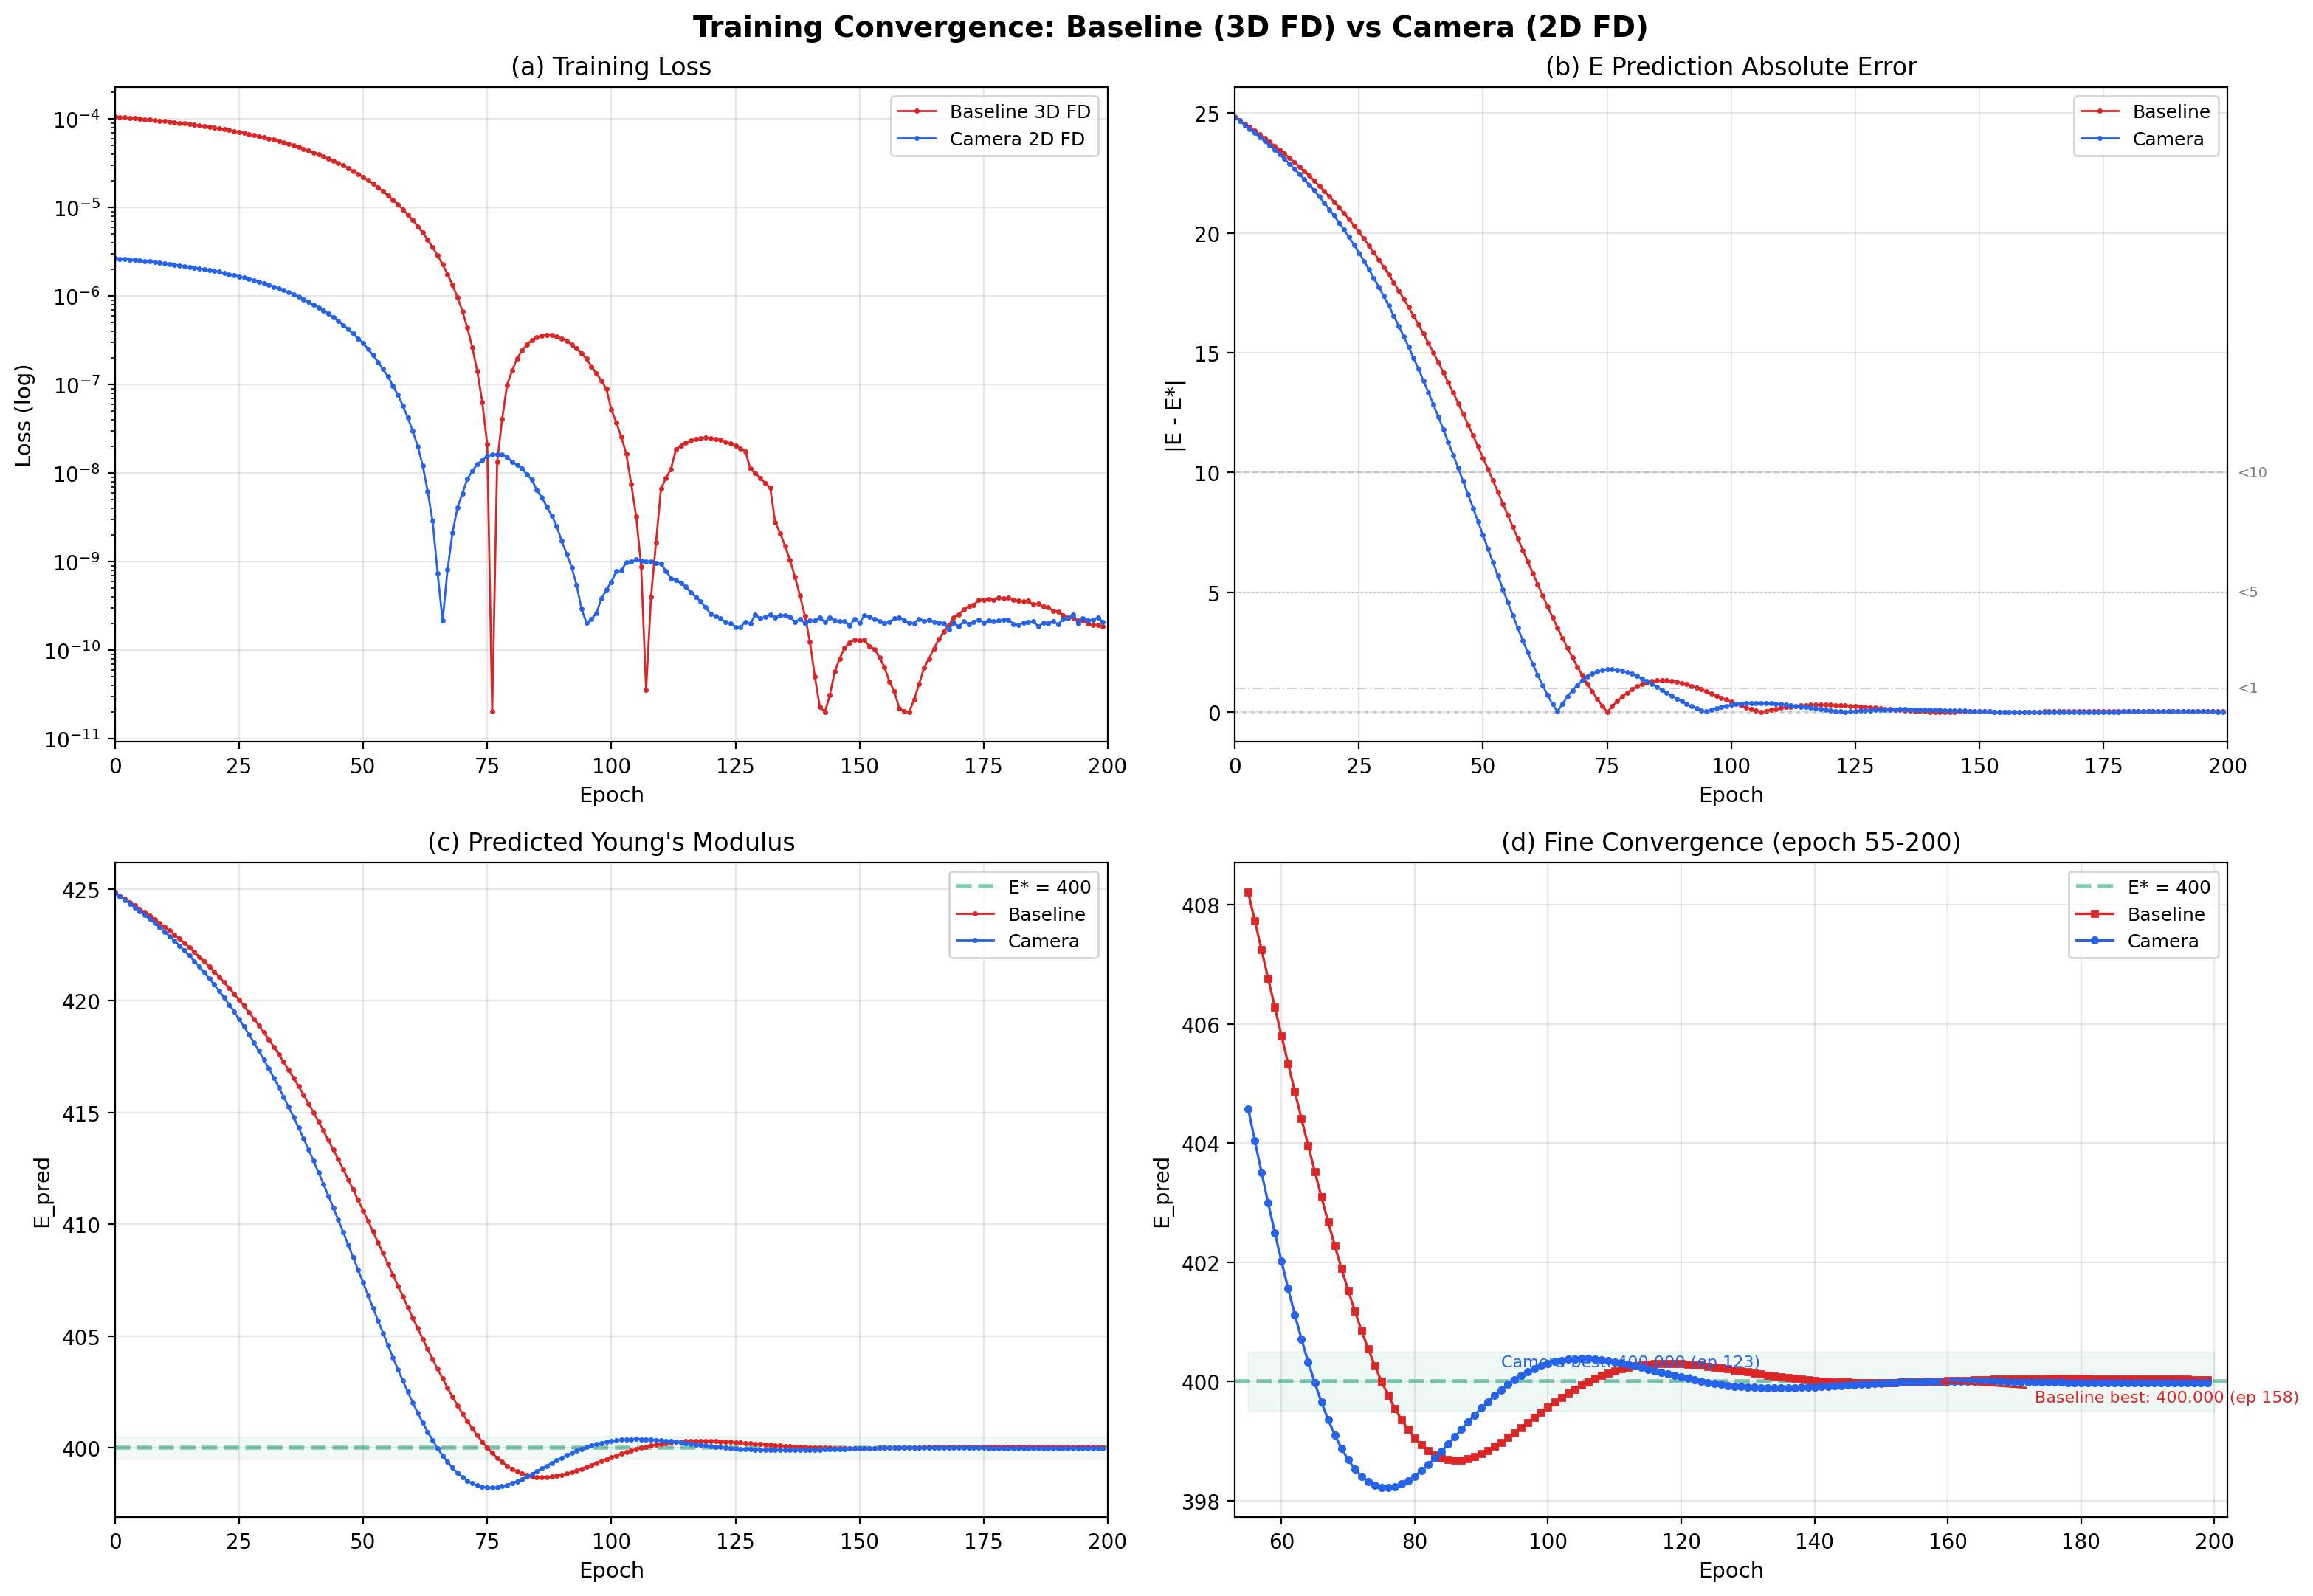
\includegraphics[width=0.96\linewidth]{fig_convergence.png}
\caption{\label{fig:convergence}Clean 3D training convergence ($E^*=400$).
(a) Loss (log scale).  (b) $|E-E^*|$ with threshold lines.
(c) $E_{\text{pred}}$ trajectory.  (d) Zoom epoch~55--200 showing oscillation
patterns.  Note: AD method not shown (failed, see Sec.~\ref{sec:ad_failure}).}
\end{figure}

\begin{figure}[H]
\centering
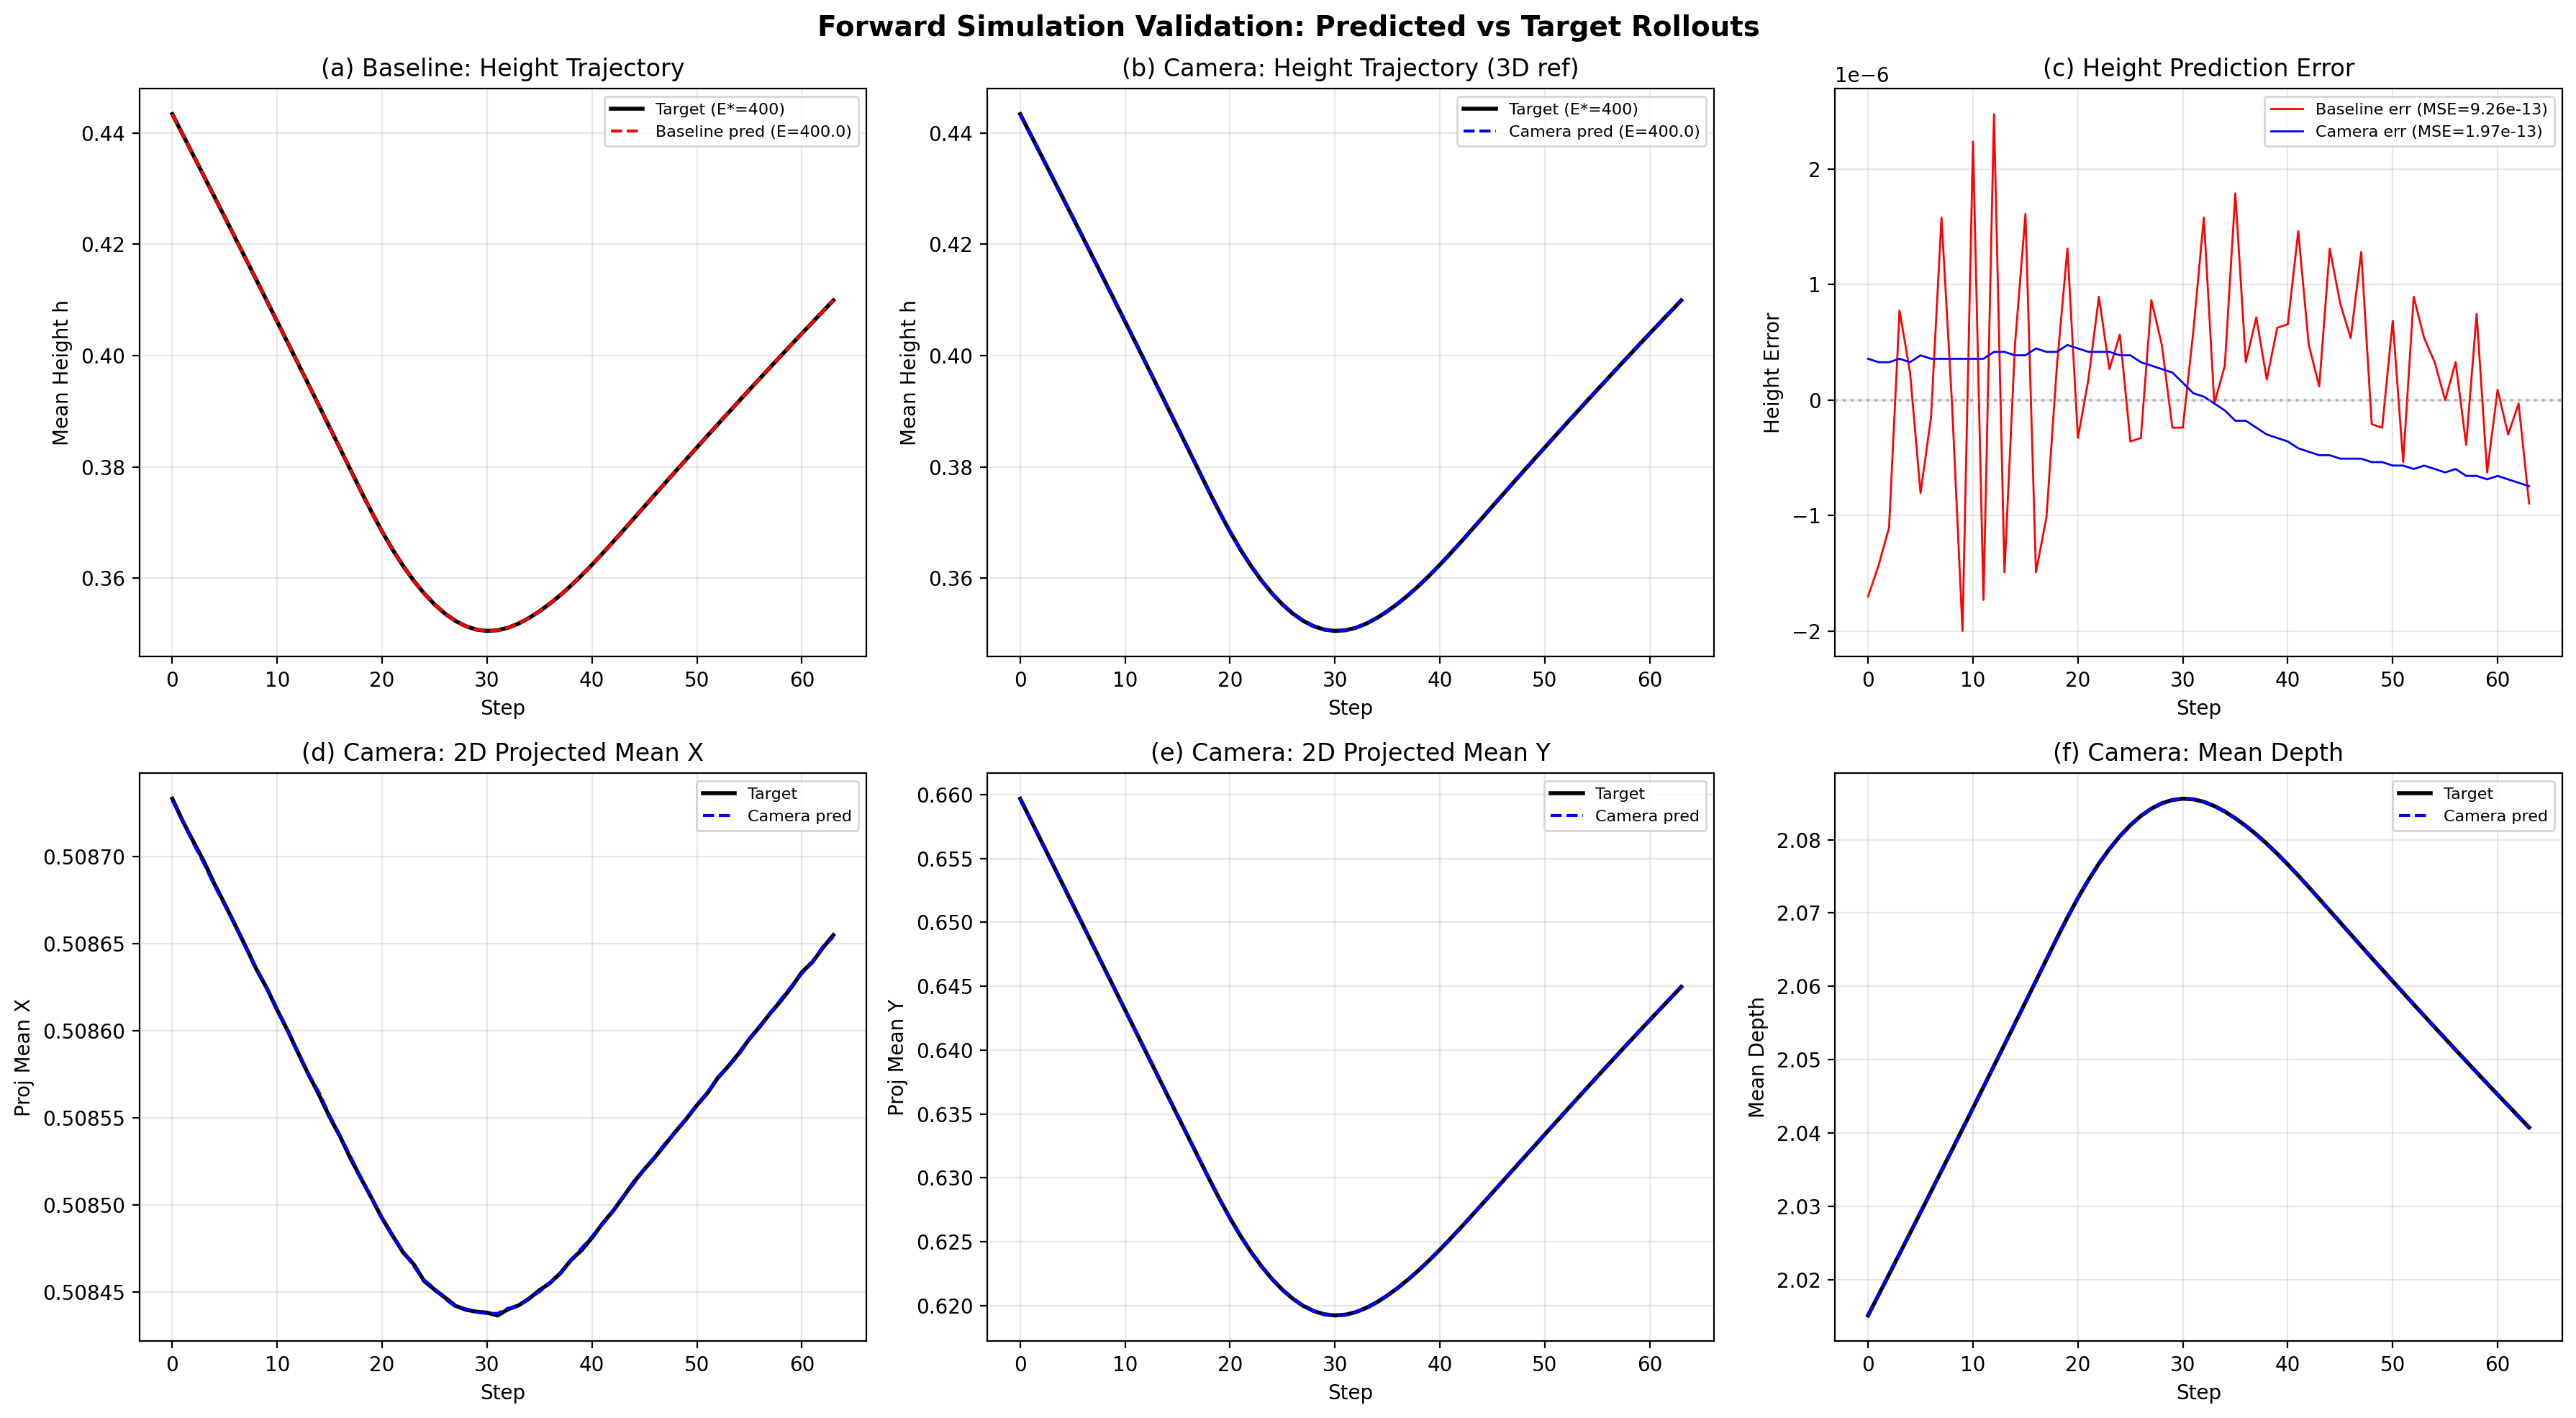
\includegraphics[width=0.95\linewidth]{fig_forward_validation.png}
\caption{\label{fig:forward}Forward simulation validation ($E^*=400$).
(a--c) 3D height trajectories---Baseline (red) and Camera (blue) vs.\ target
(black).  (d--f) Camera-space 2D observables.  All MSE values are below
$10^{-12}$, confirming physical validity of the learned $E$.}
\end{figure}

\subsection{Summary: Clean 3D Regime}

\begin{table}[H]
\centering
\caption{Clean 3D experiments summary ($E^*=400$, $\nu=0.4$ fixed).}
\label{tab:clean3d_summary}
\begin{tabular}{lccc}
\toprule
Metric & Baseline (3D FD) & Camera (2D FD) & Full AD \\
\midrule
Epochs & 200 & 200 & 100 \\
Loss initial & $1.06\times10^{-4}$ & $2.67\times10^{-6}$ & $2.57\times10^{-6}$ \\
Loss final & $1.87\times10^{-10}$ & $2.09\times10^{-10}$ & $2.57\times10^{-6}$ \\
Loss reduction & $5.68\times10^{5}\times$ & $1.28\times10^{4}\times$ & $1\times$ \\
$|E-E^*|$ final & 0.031 & \textbf{0.018} & 90.85 \\
Best $|E-E^*|$ & 0.0004 & 0.0004 & 25.09 \\
Converged ($|E-E^*|<1$) & Yes (ep~72) & Yes (ep~63) & No \\
Inference $E_{\text{pred}}$ & 400.031 & 399.982 & N/A \\
Inference MSE(h) & $9.3\times10^{-13}$ & $7.0\times10^{-13}$ & N/A \\
Per-epoch time & 0.42~s & 0.47~s & 0.08~s$^*$ \\
\bottomrule
\multicolumn{4}{l}{\footnotesize $^*$AD: $N=512$, $T=8$ (tiny mode).  Full-scale AD: NaN gradients.}
\end{tabular}
\end{table}

\textbf{Finding:} On clean 3D data, the Baseline NN+FD method reliably
recovers $E$ to high precision ($<0.03$).  The Camera variant (shown here
for reference, analyzed in depth in Sec.~\ref{sec:camera}) achieves
comparable precision with faster convergence.  Full AD is currently
infeasible on CUDA.


% ==============================================================================
\section{Experiments II: Noisy Observations (E*=450, nu*=0.35)}
\label{sec:noisy}
% ==============================================================================

We now test robustness under realistic measurement noise.  The target
switches to Regime~B ($E^*=450$, $\nu^*=0.35$) with an \emph{external-
observation} loss: only the noisy target height $h_t + \mathcal{N}(0,
\sigma^2)$ with $\sigma=10^{-3}$ is available for comparison; the
covariance and deformation-gradient channels are omitted from the loss.
This models a scenario where only a single degraded measurement channel
is accessible (e.g., noisy monocular depth estimation).

\subsection{NN+FD Under Observation Noise}

\begin{figure}[H]
\centering

\includegraphics[width=0.98\linewidth]{fig_dual_param_convergence.png}
\caption{\label{fig:noisy_convergence}NN+FD convergence under three task
conditions ($E^*=450$, $\nu^*=0.35$).  \textbf{Top row}: DualParam with
external noisy observation ($\sigma=10^{-3}$).  \textbf{Middle row}:
DualParam with clean full-observable loss.  \textbf{Bottom row}: SingleE
with clean full-observable loss (\textit{shown for comparison; analyzed in
Sec.~\ref{sec:multiparam}}).}
\end{figure}

The NN+FD method converges stably despite the noise (Fig.~\ref{fig:noisy_convergence},
top row):
\begin{itemize}[itemsep=1pt]
\item Loss drops from $8.07\times10^{-7}$ to $8.36\times10^{-8}$ ($9.6\times$
  reduction).  The smaller reduction factor reflects the noise floor.
\item $|E-E^*|$ reaches $<1$ at epoch~11, stabilizes around $0.5$--$1.5$,
  and finishes at $0.70$ (epoch~100).  The persistent oscillation is
  caused by noise-induced variance in the FD gradient: when
  $\text{Var}[L(E\pm\varepsilon)-L(E)]$ becomes comparable to the
  deterministic loss difference, the gradient direction becomes unreliable.
\item $|\nu-\nu^*|$ converges more cleanly: $<0.01$ by epoch~27, final
  $8.1\times10^{-4}$.  The $\nu$ channel appears less sensitive to
  height-only noise.
\end{itemize}

\subsection{Grid Search Baseline Under Noise}

The derivative-free grid search (Fig.~\ref{fig:nnfd_vs_baseline}) reaches
$|E-E^*|=2.78$ after 3~levels (148~evaluations) but cannot progress past
the grid resolution limit.  The noisy loss landscape has a broad,
flat-bottomed basin near $E\approx450$ that the discrete grid can
identify but not refine.

\begin{figure}[H]
\centering

\includegraphics[width=0.95\linewidth]{fig_nnfd_vs_baseline.png}
\caption{\label{fig:nnfd_vs_baseline}NN+FD vs.\ derivative-free grid search.
(a) $|E-E^*|$---NN+FD descends continuously, grid search plateaus at
$|E-E^*|\approx2.8$.  (b) $|\nu-\nu^*|$.  (c) NN+FD loss curves.
(d) Baseline $E$-vs-loss landscape.}
\end{figure}

\subsection{Forward Validation and Noise Summary}

\begin{table}[H]
\centering
\caption{Noisy experiments summary ($E^*=450$, $\nu^*=0.35$, $\sigma=10^{-3}$).}
\label{tab:noisy_summary}
\begin{tabular}{lccc}
\toprule
Metric & NN+FD & Grid Search & Clean NN+FD$^*$ \\
\midrule
Epochs / Levels & 100 & 3 & 100 \\
$|E-E^*|$ final & 0.70 & 2.78 & 0.05 \\
$|\nu-\nu^*|$ final & $8.1\times10^{-4}$ & $1.5\times10^{-3}$ & $6.3\times10^{-5}$ \\
MSE(h) inference & $8.3\times10^{-7}$ & $8.2\times10^{-7}$ & $1.9\times10^{-12}$ \\
Converged ($|E-E^*|<1$) & Yes & No & Yes \\
Forward evaluations & 300 & 148 & 300 \\
\bottomrule
\multicolumn{4}{l}{\footnotesize $^*$DualParam\_Clean, shown for reference (see Sec.~\ref{sec:multiparam}).}
\end{tabular}
\end{table}

\textbf{Finding:} NN+FD handles $\sigma=10^{-3}$ observation noise gracefully,
converging to a stable region with $|E-E^*|\approx0.7$.  The precision
ceiling is determined by the noise floor rather than optimizer behavior.
The grid search baseline identifies the general parameter region but cannot
refine past its grid resolution, demonstrating the necessity of gradient
information for precise parameter recovery under noise.


% ==============================================================================
\section{Experiments III: Camera-Space 2D Observables (E*=400)}
\label{sec:camera}
% ==============================================================================

We now evaluate the camera-space formulation (Architecture~B) in detail,
using the same $E^*=400$ target and clean data as Section~\ref{sec:clean3d},
but replacing the 3D observables with 2D projected statistics.

\subsection{Camera NN+FD Convergence}

The camera method converges faster than the 3D baseline at every threshold
(Table~\ref{tab:camera_milestones}, Fig.~\ref{fig:convergence} blue curves).
The 2D projection compresses the $8192\times3$ particle state into three
compact statistics ($\boldsymbol{\mu}_t$, $\mathbf{C}_t$, $\bar{d}_t$),
acting as an implicit regularizer that smooths the loss landscape.

\begin{table}[H]
\centering
\caption{Camera vs.\ Baseline convergence speed ($E^*=400$).}
\label{tab:camera_milestones}
\begin{tabular}{lccc}
\toprule
$|E-E^*|$ threshold & Baseline (3D FD) & Camera (2D FD) & $\Delta$ (epochs) \\
\midrule
$<20$ & 26 & 23 & $+3$ \\
$<15$ & 41 & 36 & $+5$ \\
$<10$ & 52 & 46 & $+6$ \\
$< 5$ & 62 & 55 & $+7$ \\
$< 2$ & 69 & 61 & $+8$ \\
$< 1$ & 72 & 63 & $+9$ \\
$<0.5$& 74 & 64 & $+10$ \\
$<0.1$& 75 & 65 & $+10$ \\
\midrule
Final (ep~200) & 0.031 & \textbf{0.018} & --- \\
\bottomrule
\end{tabular}
\end{table}

\subsection{Why Camera Converges Faster}

Three factors contribute:
\begin{enumerate}[itemsep=1pt]
\item \textbf{Dimensionality reduction}: $8192\times3\to3$ statistics per
  step discards high-frequency spatial modes that do not correlate with
  $E$, producing a smoother loss surface.
\item \textbf{Reduced oscillation}: the camera method oscillates with
  amplitude $\pm0.4$ near the optimum, vs.\ $\pm1.3$ for the 3D baseline
  (Fig.~\ref{fig:convergence}d).  The compressed observation space is less
  sensitive to small perturbations in $E$.
\item \textbf{Coordinate range}: 2D screen coordinates lie in $[0,1]^2$,
  bounding the observable magnitudes and preventing outlier-dominated
  loss terms.
\end{enumerate}

\subsection{Loss Scale and Stopping Criterion}

The camera loss is $\sim\!50\times$ smaller than the 3D baseline
($2.67\times10^{-6}$ vs.\ $1.06\times10^{-4}$ initially).  With the default
$|dL/dE|<10^{-8}$ stopping criterion, the camera method terminates at
epoch~64 ($|E-E^*|\approx0.32$) while the baseline continues to epoch~108
($|E-E^*|\approx0.09$).  \textbf{Disabling early stopping reveals the
camera method overtakes the baseline} (final $|E-E^*|=0.018$ vs.\ $0.031$).
Recommendation: use a \emph{relative} criterion $|dL/dE|/L<\tau$.

\subsection{Camera Forward Validation}

Forward-simulation validation (Fig.~\ref{fig:forward}, blue curves) confirms
$E_{\text{pred}}=399.982$ reproduces the target trajectory with
$\text{MSE}(\boldsymbol{\mu})=7.0\times10^{-13}$,
$\text{MSE}(\mathbf{C})=3.9\times10^{-15}$,
$\text{MSE}(\bar{d})=9.4\times10^{-12}$---comparable to the 3D baseline.

\textbf{Finding:} 2D projected statistics carry sufficient information for
precise material parameter recovery, with the additional benefits of faster
convergence and reduced post-convergence oscillation.


% ==============================================================================
\section{Experiments IV: Multi-Parameter Advanced Experiments (E*=450, nu*=0.35)}
\label{sec:multiparam}
% ==============================================================================

The final experiment section extends to dual-parameter recovery and
cross-method comparison under clean full-observable conditions.  All
experiments use Regime~B ($E^*=450$, $\nu^*=0.35$) with the complete set
of 3D observables ($h$, $\mathbf{S}$, $\bar{\mathbf{F}}$).

\subsection{Dual-Parameter NN+FD (DualParam\_Clean)}

The network simultaneously predicts $E$ and $\nu$ from the same 6-dim
input features.  Convergence (Fig.~\ref{fig:noisy_convergence}, middle row):
\begin{itemize}[itemsep=1pt]
\item Loss drops from $1.53\times10^{-4}$ to $1.56\times10^{-10}$
  ($9.81\times10^{5}\times$ reduction).
\item $|E-E^*|$ reaches $<1$ at epoch~9, $<0.5$ at epoch~9, and final
  \textbf{0.048} at epoch~100.
\item $|\nu-\nu^*|$ converges even faster: $<0.01$ by epoch~23, $<0.001$
  by epoch~24, final \textbf{$6.3\times10^{-5}$}.
\end{itemize}

The asymmetric convergence speed ($\nu$ faster than $E$) may reflect the
different sensitivity of the observables to each parameter: the position
covariance $\mathbf{S}_t$ is strongly affected by $\nu$ (which governs
volumetric locking), while $E$ primarily scales the stress magnitude.

\subsection{Single-Parameter Baseline (SingleE\_Clean)}

With $\nu$ fixed at $0.35$ and only $E$ learned, the NN+FD converges to
$|E-E^*|=0.088$ after 100 epochs (Fig.~\ref{fig:noisy_convergence},
bottom row).  The convergence is slightly slower than the dual-parameter
case ($|E-E^*|<1$ at epoch~18 vs.\ epoch~9), suggesting that jointly
learning $\nu$ provides a beneficial inductive bias---the network can
adjust $\nu$ to better fit the covariance channel, which in turn
improves the $E$ gradient signal.

\subsection{Grid Search Baseline: Gradient-Free Upper Bound}

The derivative-free grid search provides a revealing comparison
(Fig.~\ref{fig:nnfd_vs_baseline}, Table~\ref{tab:multiparam}):

\begin{itemize}[itemsep=1pt]
\item \textbf{Dual-parameter grid search}: best $|E-E^*|=2.78$,
  $|\nu-\nu^*|=1.5\times10^{-3}$ after 3~levels (148~evaluations).
  Cannot refine past grid resolution.
\item \textbf{Single-parameter line search}: best $|E-E^*|=\textbf{0.002}$
  after 24~iterations (27~evaluations)---the best result among all
  methods.  When only one parameter varies, a focused line search with
  parabolic interpolation is highly effective.
\end{itemize}

\begin{table}[H]
\centering
\caption{Multi-parameter experiments summary ($E^*=450$, $\nu^*=0.35$).}
\label{tab:multiparam}
\begin{tabular}{llccccc}
\toprule
Task & Method & Ep/It & $E_{\text{final}}$ & $|E-E^*|$ & $\nu_{\text{final}}$ & $|\nu-\nu^*|$ \\
\midrule
DualParam & NN+FD & 100 & 449.95 & \textbf{0.048} & 0.350 & \textbf{$6.3\times10^{-5}$} \\
DualParam & Grid & 3 & 452.78 & 2.78 & 0.351 & $1.5\times10^{-3}$ \\
SingleE & NN+FD & 100 & 450.09 & 0.088 & 0.350$^*$ & --- \\
SingleE & Line & 24 & 450.002 & \textbf{0.002} & 0.350$^*$ & --- \\
\midrule
\multicolumn{7}{l}{\footnotesize $^*$$\nu$ fixed (not learned).}
\end{tabular}
\end{table}

\subsection{Why Gradients Matter for Multi-Parameter Problems}

The grid search evaluates 49~discrete $(E,\nu)$ pairs per level
independently---each is a `blind' probe.  At level~3, the grid spacing
is $\Delta E\approx3.5$, $\Delta\nu\approx0.01$, placing a hard floor on
precision.  NN+FD, by contrast, uses the FD gradient to interpolate
continuously between sampled points, achieving $>50\times$ better $E$
precision with only $2\times$ the forward evaluations (300 vs.\ 148).

The single-parameter line search succeeds because: (a)~the 1D loss
landscape is convex near the optimum, (b)~each evaluation informs the
search direction, and (c)~parabolic interpolation provides a near-analytic
minimum.  These advantages vanish in $\geq 2$ dimensions, where gradient
information becomes essential.

\subsection{Forward Simulation MSE}

\begin{figure}[H]
\centering

\includegraphics[width=0.90\linewidth]{fig_forward_mse.png}
\caption{\label{fig:forward_mse}Forward simulation MSE across all Part~II
experiments.  Clean full-observable methods achieve MSE $\sim10^{-12}$;
noisy external-observation methods reach $\sim10^{-7}$.
Darker bars = NN+FD, lighter = Baseline Search.}
\end{figure}

Forward-simulation MSE (Fig.~\ref{fig:forward_mse}) confirms the parameter
estimation quality cascades to trajectory reproduction: clean dual-parameter
NN+FD achieves $\text{MSE}(h)=1.9\times10^{-12}$ while the noisy variant
reaches $8.3\times10^{-7}$---a $5\times10^{5}\times$ gap that directly
reflects the $14\times$ larger $|E-E^*|$ under noise.


% ==============================================================================
\section{Discussion}
% ==============================================================================

\subsection{Convergence Speed: 3D vs.\ 2D Camera}

The camera method's faster convergence (Table~\ref{tab:camera_milestones})
stems from implicit regularization: discarding high-frequency 3D spatial
modes removes local minima in the loss landscape that do not correlate
with $E$.  The cost is a $\sim\!50\times$ reduction in loss magnitude,
which requires attention to the stopping criterion.

\subsection{Noise Robustness}

NN+FD degrades gracefully under $\sigma=10^{-3}$ observation noise.  The
$|E-E^*|$ precision ceiling ($\approx0.7$) is determined by
$\text{Var}[\Delta L]/\varepsilon$---when the noise-induced loss variance
approaches the deterministic loss difference, the FD gradient signal-to-noise
ratio drops below 1.  Mitigation strategies include: larger $\varepsilon$
(to increase the signal), ensemble averaging of multiple FD estimates, or
using the noise-free covariance channels when available.

\subsection{Gradient Information: FD vs.\ Grid Search}

The grid search baseline demonstrates that gradient-free methods are
competitive only for 1D problems.  In the 2D $(E,\nu)$ space, the grid
search requires 148~evaluations to reach $|E-E^*|=2.78$, while NN+FD
uses 300~evaluations (100~epochs $\times$ 3~FD passes) plus 200~NN
backward passes to reach $|E-E^*|=0.048$---a $58\times$ precision
improvement.  The gradient signal effectively `interpolates' between
discrete samples in the parameter space.

\subsection{AD Failure and Path Forward}

The full AD failure is a hardware+framework limitation, not a
fundamental one.  The Taichi~1.7.4 CUDA backend struggles with deep AD
graphs involving polar decomposition; the CPU backend has a more mature
AD implementation.  For practical inverse-physics applications, the
NN+FD hybrid (Architectures~A/B) currently offers the best trade-off
between precision, memory, and numerical stability.

\subsection{Multi-View Camera Extension}

The camera method uses a single fixed viewpoint.  The modular
\texttt{Camera} class supports multiple independent instances; fusing
statistics from 2--3 cameras could recover more 3D information while
retaining the regularization benefits of 2D compression.  This is a
promising direction for future work.


% ==============================================================================
\section{Conclusion}
% ==============================================================================

We have presented a comprehensive inverse-physics learning study spanning
four experimental sections.  Key findings:

\begin{enumerate}[itemsep=2pt]
\item \textbf{Clean 3D FD works}: NN+FD reliably recovers $E$ to
  $|E-E^*|<0.03$ (and momentarily $<0.0004$) from 3D trajectory
  observables.  Full AD fails on CUDA (NaN gradients).
\item \textbf{Noise robustness}: Under $\sigma=10^{-3}$ observation noise,
  NN+FD converges stably to $|E-E^*|\approx0.7$ with a precision ceiling
  set by the noise floor.
\item \textbf{Camera acceleration}: 2D projected observables converge
  $+3$ to $+23$~epochs faster than the 3D baseline at every threshold,
  with reduced oscillation ($\pm0.4$ vs.\ $\pm1.3$).  Camera-space
  statistics are sufficient for material parameter identification.
\item \textbf{Gradient information is essential}: The grid search baseline
  plateaus at $|E-E^*|\approx2.8$ while NN+FD reaches $<0.05$.  Gradient
  access enables a $58\times$ precision improvement in dual-parameter
  recovery.
\item \textbf{Dual-parameter learning succeeds}: NN+FD simultaneously
  recovers $E$ and $\nu$ to within $6\times10^{-5}$ of their true values
  under clean conditions, with $\nu$ converging faster than $E$.
\end{enumerate}

Future work: (1) multi-camera fusion, (2) CPU-based full AD or gradient
checkpointing, (3) adaptive FD step schedules for noisy regimes,
(4) real-world soft-body video with domain transfer from simulation.


% ==============================================================================
%  Appendix
% ==============================================================================
\appendix

\section{Formulas}

\subsection{Camera Projection}
\begin{align}
\mathbf{r}_i &= \mathbf{X}_i - \mathbf{p}, \quad
d_i = -\mathbf{r}_i\cdot\mathbf{e}_z \label{eq:proj1}\\
u_i &= 0.5 + \frac{\mathbf{r}_i\cdot\mathbf{e}_x}{2d_i\tan(\theta_{\text{fov}}/2)a},
\quad v_i = 0.5 + \frac{\mathbf{r}_i\cdot\mathbf{e}_y}{2d_i\tan(\theta_{\text{fov}}/2)} \label{eq:proj2}
\end{align}

\subsection{Camera Observables}
\begin{align}
\boldsymbol{\mu}_t &= \frac{1}{N}\sum_{i=1}^N \mathbf{s}_{i,t} \in\mathbb{R}^2,
\quad \mathbf{s}_{i,t}=(u_{i,t}, v_{i,t}) \label{eq:mean}\\
\mathbf{C}_t &= \frac{1}{N}\sum_{i=1}^N (\mathbf{s}_{i,t}-\boldsymbol{\mu}_t)(\mathbf{s}_{i,t}-\boldsymbol{\mu}_t)^\top \in\mathbb{R}^{2\times2} \label{eq:cov}\\
\bar{d}_t &= \frac{1}{N}\sum_{i=1}^N d_{i,t} \in\mathbb{R} \label{eq:depth}
\end{align}

\subsection{Loss Functions}
\begin{align}
L_t^{\text{3D}} &= \frac{1}{T}\Big((h_t^{\text{pred}}-h_t^{\text{target}})^2
    + 10\lVert\mathbf{S}_t^{\text{pred}}-\mathbf{S}_t^{\text{target}}\rVert_F^2
    + 5\lVert\bar{\mathbf{F}}_t^{\text{pred}}-\bar{\mathbf{F}}_t^{\text{target}}\rVert_F^2\Big)\\
L_t^{\text{cam}} &= \frac{1}{T}\Big(100\lVert\boldsymbol{\mu}_t^{\text{pred}}-\boldsymbol{\mu}_t^{\text{target}}\rVert^2
    + 500\lVert\mathbf{C}_t^{\text{pred}}-\mathbf{C}_t^{\text{target}}\rVert_F^2
    + 10(\bar{d}_t^{\text{pred}}-\bar{d}_t^{\text{target}})^2\Big) \label{eq:camloss}
\end{align}

\section{Full Experiment Results Table}

\begin{table}[H]
\centering
\caption{Complete experiment summary across all 4 sections.}
\label{tab:full_results}
{\small
\begin{tabular}{llcccccc}
\toprule
Section & Task & Method & Ep/It & $|E-E^*|$ & $|\nu-\nu^*|$ & MSE(h) & Conv. \\
\midrule
\S\ref{sec:clean3d} & Clean 3D (400) & Baseline FD & 200 & 0.031 & --- & $9.3\times10^{-13}$ & Yes \\
\S\ref{sec:clean3d} & Clean 3D (400) & Camera FD & 200 & \textbf{0.018} & --- & $7.0\times10^{-13}$ & Yes \\
\S\ref{sec:clean3d} & Clean 3D (400) & Full AD & 100 & 90.85 & --- & N/A & No \\
\midrule
\S\ref{sec:noisy} & Noisy (450) & NN+FD & 100 & 0.70 & $8.1\times10^{-4}$ & $8.3\times10^{-7}$ & Yes \\
\S\ref{sec:noisy} & Noisy (450) & Grid & 3 & 2.78 & $1.5\times10^{-3}$ & $8.2\times10^{-7}$ & No \\
\midrule
\S\ref{sec:camera} & Camera (400) & Camera FD & 200 & \textbf{0.018} & --- & $7.0\times10^{-13}$ & Yes \\
\midrule
\S\ref{sec:multiparam} & Dual (450) & NN+FD & 100 & 0.048 & \textbf{$6.3\times10^{-5}$} & $1.9\times10^{-12}$ & Yes \\
\S\ref{sec:multiparam} & Dual (450) & Grid & 3 & 2.78 & $1.5\times10^{-3}$ & $1.1\times10^{-9}$ & No \\
\S\ref{sec:multiparam} & SingleE (450) & NN+FD & 100 & 0.088 & --- & $2.1\times10^{-12}$ & Yes \\
\S\ref{sec:multiparam} & SingleE (450) & Line & 24 & \textbf{0.002} & --- & $1.0\times10^{-12}$ & Yes \\
\bottomrule
\end{tabular}}
\end{table}

\section{NN Input Features}

\subsection*{3D Baseline ($d=6$)}
$z_0=h_0$, $z_1=h_{T-1}$, $z_2=\max(h)-\min(h)$,
$z_3=\frac{1}{T}\sum_t\operatorname{tr}(\mathbf{S}_t)$,
$z_4=\max_t\operatorname{tr}(\mathbf{S}_t)$,
$z_5=|h_{T-1}-h_0|/(T\cdot s\cdot\Delta t)$.

\subsection*{Camera ($d=8$)}
$z_0=\mu_{u,0}$, $z_1=\mu_{v,0}$, $z_2=\mu_{u,T-1}$, $z_3=\mu_{v,T-1}$,
$z_4=\frac{1}{T}\sum_t\operatorname{tr}(\mathbf{C}_t)$,
$z_5=\max_t\operatorname{tr}(\mathbf{C}_t)$,
$z_6=\max(\bar{d})-\min(\bar{d})$,
$z_7=|\mu_{v,T-1}-\mu_{v,0}|/(T\cdot s\cdot\Delta t)$.

\section{Code and Data Availability}

\begin{itemize}[itemsep=0pt]
\item \texttt{Inversive/code/} --- source code (simulation, NN, camera, training)
\item \texttt{Inversive/data*/} --- training logs and predicted trajectories
\item \texttt{experiments\_results.csv} --- Clean 3D + Camera data (546~rows)
\item \texttt{report/experiment\_results\_formatted.csv} --- Noisy + Multi-param data (743~rows)
\end{itemize}

\bibliographystyle{alpha}
\bibliography{sample}

\end{document}
